\documentclass[parskip=full]{scrartcl}
\usepackage[utf8]{inputenc}
\usepackage[T1]{fontenc}
\usepackage[ngerman]{babel}
\usepackage{enumerate}
\usepackage{enumitem}
\usepackage{hyperref}
\usepackage{graphicx}
\usepackage{float}
\usepackage{lmodern}
\usepackage{csquotes}
\usepackage[toc]{glossaries}
\usepackage{array}

\setlist[enumerate]{itemsep=-2.5mm}
\setlist[enumerate,2]{label=\arabic*.}
\setlist[description]{itemsep=-2.5mm}
\newcommand{\req}[1]{\mbox{/#1/}}

\title{ContentBasedBrowser -CoBaB- \\ Qualitätssicherung}
\hypersetup{
    colorlinks,
    citecolor=black,
    filecolor=black,
    linkcolor=black,
    urlcolor=black
}

\renewcommand{\glossarysection}[2][]{}
%\makeglossaries
%\newglossaryentry{Annotation}
{
name=Annotation,
description={ist ein in den Datensätzen vordefinierter Bereich eines Bildes oder Videos}
}

\newglossaryentry{Lesezeichen}
{
name=Lesezeichen,
description={ist ein Link für schnelleren Zugriff auf bestimmte, meist häufig besuchte Ergebnisse in einer Lesezeichen-Sammlung}
}

\newglossaryentry{Chronik}
{
name=Chronik,
description={ist eine Sammlung von gespeicherten zuletzt besuchten Seiten im Programm. \newline Wird als Synonym von Historie im Dokument verwendet}
}

\newglossaryentry{Feedback}
{
name=Feedback,
description={umfasst das Bewerten der generierten Ergebnisse und ihr Witerleiten an den Suchalgorithmen für eine verbesserte Suche}
}



\newglossaryentry{GUI}
{
name=GUI,
description={(engl. graphical user interface) Grafische Benutzeroberfläche}
}

\newglossaryentry{Dialog}
{
name=Dialog,
description={ist ein Element der grafischen Benutzeroberfläche, bei dem Eingaben vom Benutzer eingeholt werden}
}

\newglossaryentry{Versionsverwaltung}
{
name=Versionsverwaltung,
description={Versionsverwaltung ist ein System, dass Änderungen an Dateien erfasst und mit einem Zeitstempel dokumentiert, um beliebige vorherige Versionen wiederherzustellen. Der Gebrauch von Versionsverwaltung heißt Versionierung}
}

\newglossaryentry{Git}
{
name=Git,
description={ist eine freie Software zur Versionsverwaltung von Dateien}
}

\newglossaryentry{Phase}
{
name=Phase,
description={ist einer der Abschnitte im Verlauf der Entwicklung eines Softwareprodukts: Planung, Entwurf, Implementierung, Testen, Wartung und Pflege}
}

\newglossaryentry{Phasendokument}
{
name=Phasendokument,
description={ist das Resultat einer Phase der Softwareentwicklung}
}

\newglossaryentry{Qt}
{
name=Qt,
description={ist eine Klassenbibliothek, also eine Sammlung von Routinen und Hilfsmitteln in Form von Programmcode, die die Darstellung von grafischen Benutzeroberflächen erlaubt. Sie ist in der Programmiersprache C++ verfasst}
}

\newglossaryentry{Qt Creator}
{
name=Qt Creator,
description={ist eine integrierte Entwicklungsumgebung - ein Hilfsmittel bei der Erstellung von Programmcode}
}

\newglossaryentry{Qt Designer}
{
name=Qt Designer,
description={ist ein Hilfsmittel zum Entwerfen und Erstellen grafischer Benutzeroberflächen}
}

\newglossaryentry{Qt Test}
{
name=Qt Test,
description={ist eine Framework für Modultests - ein Hilfsmittel beim kontinuierlichen Testen eines Programms bereits während der Implementierung}
}

\newglossaryentry{Suchverfahren}
{
name=Suchverfahren,
description={ist eine Routine, die die Bilder bzw. Videos eines gegebenen Datensatzes in ihrer Ähnlichkeit mit einer gegebenen Suchvorlage bewertet. \newline Wird als Synonym von Suchalgorithmen im Dokument verwendet.}
}

\newglossaryentry{Widget}
{
name=Widget,
description={ist eine verallgemeinernde Bezeichnung für Komponenten eines GUI}
}

\newglossaryentry{Entwurfsmuster}
{
name=Entwurfsmuster,
description={ist eine Lösung für häufig auftretende Probleme beim Entwurf von Software}
}

\newglossaryentry{Model-View-Controller}
{
name=Model-View-Controller,
description={ist ein Muster zur Strukturierung von Software-Entwicklung in die drei Einheiten Datenmodell (engl. model), Präsentation (engl. view) und Programmsteuerung (engl. controller). Ziel des Musters ist ein flexibler Programmentwurf, der eine spätere Änderung oder Erweiterung erleichtert und eine Wiederverwendbarkeit der einzelnen Komponenten ermöglicht.}
}

\newglossaryentry{Doxygen}
{
name=Doxygen,
description={ist eine freie Software, die aus Quellcode und darin enthaltenen Kommentaren eine Softwaredokumentation erzeugt}
}


\begin{document}
\begin{titlepage}
\title{ContentBasedBrowser -CoBaB- \\ Qualitätssicherung}
\author{Anja Blechinger, Marie Bommersheim, Georgi Georgiev,\\ Tung Nguyen, Vincent Winkler, Violina Zhekova}
\date{März 2016}
\maketitle
\vspace{300pt}
\begin{tabular}{l l}
Projekt: & Media Browser zur inhaltsbasierten Suche in Bild- und Videodaten\\
Auftraggeber: & Arne Schumann,\\
 & Fraunhofer Institut für Optronik, Systemtechnik und Bildauswertung,\\
 & Karlsruhe\\
\end{tabular}
\thispagestyle{empty}
\end{titlepage}
\setcounter{page}{1}

\tableofcontents
\pagebreak

\section{Einleitung}
In diesem Dokument wird die Qualitätssicherung von CoBaB beschrieben. \newline
Die Aufgabe dieser Phase ist es, die Bedienbarkeit und Funktionalität von CoBaB zu testen und eventuelle Fehler zu beheben. Dies ermöglichen die im Pflichtenheft beschriebenen und weitere Testszenarien. \newline
Außerdem wird überprüft, wie viel des erarbeiteten Codes durch die Testfälle abgedeckt wird. 
\pagebreak

\section{Testszenarien}
% !TeX spellcheck = de_DE_frami
\subsection{Testdaten}
Zum Testen während der Entwicklung und zum Durchspielen der Testszenarien werden mindestens nachfolgende Testdaten benötigt:
\begin{itemize}
	\item ein Bilddatensatz (mit mehreren Bildern und mindestens einem annotiertem Bild)
	\item ein Datensatz mit mindestens einem Video aus Einzelbildern
	\item ein Testsuchverfahren, das eine beliebige Sortierung als Suchergebnis zurück gibt
	\item ein Suchverfahren, das auf eine Annotation des oben geforderten annotierten Bildes anwendbar ist
\end{itemize}
Insbesondere die Schnittstelle zwischen Suchverfahren und Anwendung soll durch diese Testdaten überprüft werden.

\subsection{Testszenarien}
Die folgenden Testszenarien sind dem Pflichtenheft entnommen und beschreiben den Arbeitsablauf des Benutzers im Detail.

\subsubsection{Testszenarien der Pflichtanforderungen}
\begin{enumerate} [label=\bfseries /TS \arabic*0/, leftmargin=*]
	\item Grundfunktionalität \newline \newline
	\begin{tabular}{rp{4in}|l}
	1. & \textbf{Vorbedingung} Das Programm ist startbereit; es wurden weder Datensätze noch Suchverfahren entfernt oder manipuliert & \\
	   & \textbf{Aktion} Der Benutzer startet das Programm &  \\
	   & \textbf{Nachbedingung} Die Startansicht der GUI wird angezeigt; die Bibliothek wird angezeigt und enthält alle Datensätze des Standardordners & bestanden \\
	\hline
	2. & \textbf{Aktion} Der Benutzer doppelklickt einen Datensatz & \\
	   & \textbf{Nachbedingung} Es wird eine Übersicht des Datensatzes angezeigt & bestanden \\
	\end{tabular}	   
	\begin{tabular}{rp{4in}|l}
	3. & \textbf{Aktion} Der Benutzer klickt auf ein Bild aus der Übersicht & \\
	   & \textbf{Nachbedingung} Das Bild wird groß dargestellt & bestanden \\
	\hline    
    4. & \textbf{Aktion} Der Benutzer rechtsklickt auf einen Bereich des Bildes, der nicht annotiert ist & \\
       & \textbf{Nachbedingung} Es wird ein Kontextmenü angezeigt, in dem mindestens ein Suchverfahren zur Auswahl bereitsteht & bestanden \\
	\hline    
    5. & \textbf{Aktion} Der Benutzer fährt mit der Maus über ein Suchverfahren & \\
	   & \textbf{Nachbedingung} Es wird eine Beschreibung des Suchverfahrens angezeigt & bestanden \\
	\hline    
    6. & \textbf{Aktion} Der Benutzer linksklickt auf eines der Suchverfahren & \\
	   & \textbf{Nachbedingung} Das angezeigte Fenster enthält die Parameter des Suchverfahrens und entsprechende UI-Elemente, die ermöglichen sie festzulegen & bestanden \\
	\hline	
	7. & \textbf{Aktion} Der Benutzer nimmt seine Eingaben vor und bestätigt sie & \\
	   & \textbf{Nachbedingung} Es werden die vorgenommenen Einstellungen angezeigt; eine Schaltfläche zum Starten der Suche wird angezeigt & bestanden \\
	\hline    
    8. & \textbf{Aktion} Der Benutzer startet die Suche & \\
       & \textbf{Nachbedingung} Eine Animation zeigt die Aktivität des Suchverfahrens an & bestanden \\
	\hline	
	9. & \textbf{Aktion} Der Benutzer wartet & \\
       & \textbf{Nachbedingung} Eine Übersicht über die Ergebnisse der Suche wird angezeigt & bestanden \\
	\hline   
   10. & \textbf{Aktion} Der Benutzer wählt die Schaltfläche zur Rückkehr & \\
	   & \textbf{Nachbedingung} Es werden wieder die vorgenommenen Einstellungen angezeigt; eine Schaltfläche zum Starten der Suche wird angezeigt & bestanden \\
	\hline
   11. & \textbf{Aktion} Der Benutzer startet die Suche erneut & \\
	   & \textbf{Nachbedingung} Eine Animation zeigt die Aktivität des Suchverfahrens an & bestanden \\
	\hline   
   12. & \textbf{Aktion} Der Benutzer beendet das Programm (während der laufenden Suche) über den üblichen Schließen-Button & \\ 
	   & \textbf{Nachbedingung} die GUI ist nicht mehr sichtbar; der Prozess hat terminiert & bestanden \\
	\end{tabular}
	
	\pagebreak

	\item Kommandozeile \newline \newline
	\begin{tabular}{rp{4in}|l}
	1. & \textbf{Vorbedingung} Das Programm ist startbereit & \\
	   & \textbf{Aktion} Der Benutzer startet das Programm mit einem Pfad als Kommandozeilenargument in der entsprechenden Position & \\
	   & \textbf{Nachbedingung} In der Bibliothek werden die Datensätze, die sich an dem übergebenen Pfad befinden, angezeigt & bestanden \\
	\hline	
	2. & \textbf{Aktion} Der Benutzer wählt über den Menüpunkt ganz rechts \enquote{Hilfe} aus & \\
	   & \textbf{Nachbedingung} Ein Dialog mit Hinweisen zur Benutzung des Programms wird angezeigt & bestanden \\
	\end{tabular}
	\newline

	\item erweiterte Funktionen zu Bilddatensätzen \newline \newline
	\begin{tabular}{rp{4in}|l}
	1. & \textbf{Vorbedingung} Es wurde ein Datensatz (bestehend aus Bildern) gewählt; das Programm zeigt die Übersicht der Bilder des Datensatzes; es ist ein Foto eines realen Motivs im Datensatz vorhanden; das Foto weist annotierte Bildbereiche auf & \\
	   & \textbf{Aktion} Der Benutzer wählt dieses Bild zur vergrößerten Ansicht & \\
	   & \textbf{Nachbedingung} Das Bild wird in vergrößerter Ansicht angezeigt; es werden die annotierten Bildbereiche angezeigt & bestanden \\
	\hline
	2. & \textbf{Aktion} Der Benutzer verwendet die Schaltflächen, um zum nächsten und vorherigen Bild zu wechseln & \\
	   & \textbf{Nachbedinung} Das Bild in der größeren Ansicht wechselt vor bzw. zurück entsprechend der durch die Übersicht gegebenen Reihenfolge & bestanden \\
	\hline
	3. & \textbf{Aktion} Der Benutzer kehrt zum annotierten Bild zurück; der Benutzer rechtsklickt auf einen annotierten Bildbereich & \\
	   & \textbf{Nachbedingung} Es wird ein Kontextmenü angezeigt, in dem mindestens ein Suchverfahren zur Auswahl bereitsteht & bestanden \\
	\hline
	4. & \textbf{Aktion} Der Benutzer linksklickt auf ein Suchverfahren & \\
	   & \textbf{Nachbedingung} Es wird die Parameterauswahl angezeigt & bestanden \\
	\hline
	5. & \textbf{Aktion} Der Benutzer wählt seine Parameter und bestätigt sie & \\
	   & \textbf{Nachbedingung} Es wird der gewählte annotierte Bildbereich angezeigt; eine Schaltfläche zur Rückkehr zur Parameterauswahl wird angezeigt & bestanden \\
	\end{tabular}
	
	\begin{tabular}{rp{4in}|l}
	6. & \textbf{Aktion} Der Benutzer linksklickt die Schaltfläche zur Rückkehr zweimal & \\
	   & \textbf{Nachbedingung}	Das eben gewählte Bild wird in der vergrößerten Ansicht dargestellt & nicht bestanden\\
	\hline
	7. & \textbf{Aktion} Der Benutzer wählt das Werkzeug zur Auswahl eines Bildbereiches und wählt per Drag-and-Drop in der vergrößerten Ansicht einen Bildbereich & \\
	   & \textbf{Nachbedingung} Der gewählte Bereich wird dargestellt & bestanden \\
	\hline	
	8. & \textbf{Aktion} Der Benutzer rechtsklickt in den gewählten Bereich und linksklickt auf ein Suchverfahren & \\
	   & \textbf{Nachbedingung} Es wird die Parameterauswahl angezeigt & bestanden \\
	\hline	
	9. & \textbf{Aktion} Der Benutzer wählt seine Parameter und bestätigt sie & \\
	   & \textbf{Nachbedingung} Es wird der gewählte Bildbereich angezeigt; eine Schaltfläche zur Rückkehr zur Parameterauswahl wird angezeigt & bestanden \\
	\hline   
   10. & \textbf{Aktion} Der Benutzer linksklickt die Schaltfläche zur Rückkehr zweimal & \\
	   & \textbf{Nachbedingung} Das eben gewählte Bild wird in der vergrößerten Ansicht dargestellt; der gewählte Bildbereich wird angezeigt & nicht bestanden \\
	\hline
   11. & \textbf{Aktion} Der Benutzer verwendet die Schaltflächen, um zum nächsten und vorherigen Bild zu wechseln & \\
	   & \textbf{Nachbedingung} Das Bild in der größeren Ansicht wechselt vor bzw. zurück entsprechend der durch die Übersicht gegebenen Reihenfolge & bestanden \\
	\hline
   12. & \textbf{Aktion} Der Benutzer linksklickt die Schaltfläche zur Rückkehr zur Bibliothek & \\
	   & \textbf{Nachbedingung} Die Bibliothek wird angezeigt & bestanden \\
	\end{tabular}
	\newline

	\item Feedback und weitere Suche \newline \newline
	\begin{tabular}{rp{4in}|l}
	1. & \textbf{Vorbedingung} Das Programm zeigt die Ergebnisse einer Suche & \\
	   & \textbf{Aktion} Der Benutzer stellt für mehrere Ergebnisse ein Feedback ein & \\
	   & \textbf{Nachbedingung}Das eingestellte Feedback wird dargestellt & bestanden \\
	\hline	
	2. & \textbf{Aktion} Der Benutzer startet über die entsprechende Schaltfläche eine weitere Suche und wartet & \\
	   & \textbf{Nachbedingung} Die Ergebnisse werden angezeigt & bestanden \\
	 \end{tabular}
	 \pagebreak

	\item Datensatz zur Bibliothek hinzufügen \newline \newline
	\begin{tabular}{rp{4in}|l}
	1. & \textbf{Vorbedingung} Programm ist startbereit; ein korrekter Datensatz liegt auf der Festplatte & \\
	   & \textbf{Aktion} Benutzer startet Programm & \\
	   & \textbf{Nachbedingung} Startbildschirm der GUI wird angezeigt; die Bibliothek wird angezeigt & bestanden \\
	\hline	
	2. & \textbf{Aktion} Der Benutzer klickt die Schaltfläche zum Hinzufügen eines neuen Datensatzes & \\
	   & \textbf{Nachbedingung} Ein Dialog, der die Auswahl eines Datensatzes von der Festplatte ermöglicht, wird angezeigt & bestanden \\
	\hline	
	3. & \textbf{Aktion} Der Benutzer wählt einen korrekten Datensatz von der Festplatte und bestätigt seine Wahl & \\
	   & \textbf{Nachbedingung} Der Dialog wird nicht mehr angezeigt; es wird eine Übersicht des gewählten Datensatzes angezeigt & bestanden \\
	\hline	
	4. & \textbf{Aktion} Der Benutzer linksklickt die Schaltfläche zur Rückkehr & \\
	   & \textbf{Nachbedingung} Die Liste der Bibliothek enthält den eben gewählten Datensatz & bestanden \\
	\end{tabular}
	\newline

	\item Videos aus Einzelbildern abspielen \newline \newline
	\begin{tabular}{rp{4in}|l}
	1. & \textbf{Vorbedingung} Es wurde ein Datensatz gewählt, der mindestens ein Video aus Einzelbildern enthält & \\
	   & \textbf{Aktion} Der Benutzer wählt eines der Videos zur Ansicht & \\
	   & \textbf{Nachbedingung} Ein Videoplayer wird angezeigt; eine Schaltfläche zum Starten des Videos ist verfügbar & bestanden \\
	\hline
	2. & \textbf{Aktion} Der Benutzer klickt auf die Schaltfläche zum Starten des Videos & \\
	   & \textbf{Nachbedingung} Das Video wird abgespielt & bestanden \\
	\end{tabular}
	\newline

	\item weitere Menüpunkte \newline \newline
	\begin{tabular}{rp{4in}|l}
	1. & \textbf{Vorbedingung} Das Menü ist verfügbar & \\
	   & \textbf{Aktion} Der Benutzer wählt über den Menüpunkt ganz rechts \enquote{About} aus & \\
	   & \textbf{Nachbedingung} Ein Dialog mit Informationen zum Programm wird angezeigt & bestanden \\
	\hline
	2. & \textbf{Aktion} Der Benutzer wählt über den Menüpunkt ganz rechts \enquote{Hilfe} aus & \\
	   & \textbf{Nachbedingung} Ein Dialog mit Hinweisen zur Benutzung des Programms wird angezeigt & bestanden \\
	\end{tabular}
	\newline

	\newpage
	Die folgenden Testszenarien kamen erst in der Testphase hinzu.

	\item Interaktion mit Videos aus Einzelbildern \newline \newline
	\begin{tabular}{rp{4in}|l}
	1. & \textbf{Vorbedingung} Es gibt einen Datensatz mit mind. zwei SingleFrameVideos & \\
	   & \textbf{Aktion} Wähle diesen Datensatz & \\
	   & \textbf{Nachbedingung} Es wird eine Übersicht der Videos angezeigt, das erste Video wird groß dargestellt & bestanden \\
	\hline
	2. & \textbf{Aktion} Wähle ein Video und starte es mithilfe des Play Buttons & \\
	   & \textbf{Nachbedingung} Das ausgewählte Video wird abgespielt, der Slider bewegt sich & bestanden \\
	\hline
	3. & \textbf{Aktion} Wähle währenddessen ein anderes Video und starte es & \\
	   & \textbf{Nachbedingung} Das ausgewählte Video wird angezeigt und abgespielt & bestanden \\
	\hline
	4. & \textbf{Aktion} Pausiere das Video mithilfe des Pause Buttons & \\
	   & \textbf{Nachbedingung} Das Video pausiert & bestanden \\
	\hline
	5. & \textbf{Aktion} Klicke den Play Button & \\
	   & \textbf{Nachbedingung} Das Video wird weiter abgespielt & bestanden \\
	\hline
	6. & \textbf{Aktion} Klicke den Stop Button & \\
	   & \textbf{Nachbedingung} Das Video wird gestoppt & bestanden \\
	\hline
	7. & \textbf{Aktion} Klicke den Play und anschließend den Loop Button & \\
	   & \textbf{Nachbedingung} Das Video wird abgespielt und nach dem Ende erneut abgespielt & bestanden \\
	\hline
	8. & \textbf{Aktion} Zoome in das Video hinein und wieder hinaus & \\
	   & \textbf{Nachbedingung} Es wird während des Abspielens in das Video hinein/heraus gezoomt & bestanden \\
	\hline
	9. & \textbf{Aktion} Klicke den Loop Button & \\
	   & \textbf{Nachbedingung} Das Video wird nach dem Ende nicht erneut abgespielt & bestanden \\
	\hline
	10. & \textbf{Aktion} Klicke den Play Button & \\
	    & \textbf{Nachbedingung} Das Video wird abgespielt & bestanden \\
	\hline
	11. & \textbf{Aktion} Rechtsklicke auf eine Annotation im laufenden Video & \\
	    & \textbf{Nachbedingung} Das Video pausiert und es wird ein Kontextmenü angezeigt, das die verfügbaren Suchverfahren anzeigt & bestanden \\
	\hline
	12. & \textbf{Aktion} Wähle ein Suchverfahren und die Parameter und klicke auf \enquote{Weiter} & \\
	    & \textbf{Nachbedingung} Die gewählte Annotation wird im Überprüfungsfenster angezeigt & bestanden \\
	\end{tabular}
	\newline

	\newpage
	\item Navigation \newline \newline
	\begin{tabular}{rp{4in}|l}
	1. & \textbf{Vorbedingung} Der Viewer ist sichtbar & \\
	   & \textbf{Aktion} Wähle den Home Button & \\
	   & \textbf{Nachbedingung} Die Library wird angezeigt & bestanden \\
	\hline
	2. & \textbf{Aktion} Wähle einen Datensatz und einen Algorithmus; Klicke den Home Button & \\
	   & \textbf{Nachbedingung} Die Library wird angezeigt & bestanden \\
	\hline
	3. & \textbf{Aktion} Wähle einen Datensatz, einen Algorithmus und die Parameter; Klicke den Home Button & \\
	   & \textbf{Nachbedingung} Die Library wird angezeigt & bestanden \\
	\hline
	4. & \textbf{Aktion} Wähle einen Datensatz, einen Algorithmus, die Parameter und starte die Suche; klicke während der laufenden Suche den Home Button & \\
	   & \textbf{Nachbedingung} Die Library wird angezeigt & bestanden \\
	\hline
	5. & \textbf{Vorbedingung} Das Ergebnisfenster wird angezeigt & \\
	   & \textbf{Aktion} Klicke den zurück Button & \\
	   & \textbf{Nachbedingung} Das Bestätigungfenster wird angezeigt & bestanden \\
	\hline
	6. & \textbf{Aktion} Klicke den zurück Button & \\
	   & \textbf{Nachbedingung} Das Parameterauswahl wird angezeigt & bestanden \\
	\hline
	7. & \textbf{Aktion} Klicke den zurück Button & \\
	   & \textbf{Nachbedingung} Der Viewer wird angezeigt & bestanden \\
	\hline
	8. & \textbf{Aktion} Klicke den zurück Button & \\
	   & \textbf{Nachbedingung} Die Library wird angezeigt & bestanden \\
	\end{tabular}

\end{enumerate}

\newpage

\subsubsection{Testszenarien der Wunschanforderungen}
\begin{enumerate} [label=\bfseries /TSW \arabic*0/, leftmargin=*]
	\item Feedback, Suchchronik und Lesezeichen \newline \newline
	\begin{tabular}{rp{4in}|l}
	1. & \textbf{Vorbedingung} Es wurde gerade eine Suche durchgeführt; es werden die Ergebnisse der Suche angezeigt & \\
	   & \textbf{Aktion} Der Benutzer stellt ein positives und ein negatives Feedback für je ein Suchergebnis ein & \\
	   & \textbf{Nachbedingung} Das gegebene Feedback wird in der Übersicht dargestellt & bestanden \\
	\hline
	2. & \textbf{Aktion} Der Benutzer beendet das Programm & \\
	   & \textbf{Nachbedingung} Das Programm wurde beendet & bestanden \\
	\hline
	3. & \textbf{Aktion} Der Benutzer startet das Programm erneut & \\
	   & \textbf{Nachbedingung} Die Startansicht der GUI wird angezeigt & bestanden \\
	\hline	
	4. & \textbf{Aktion} Der Benutzer wählt den Menüpunkt \enquote{Chronik} & \\
	   & \textbf{Nachbedingung} Die zuletzt beendeten Suchen werden angezeigt & nicht bestanden \\
	\hline
	5. & \textbf{Aktion} Der Benutzer wählt die zuletzt beendete Suche & \\
	   & \textbf{Nachbedingung} Die bereits zuvor angezeigten Suchergebnisse werden in der selben Reihenfolge wieder angezeigt; das zuvor festgelegte Feedback wird wieder angezeigt & nicht bestanden \\
	\hline
	6. & \textbf{Aktion} Der Benutzer klickt auf die Schaltfläche zum Speichern der Suchergebnisse, gibt einen Namen für das Lesezeichen ein und beendet anschließend das Programm & \\
	   & \textbf{Nachbedingung} Das Programm wurde beendet & nicht bestanden \\
	\hline
	7. & \textbf{Aktion} Der Benutzer startet das Programm erneut & \\
	   & \textbf{Nachbedingung} Die Startansicht der GUI wird angezeigt & bestanden \\
	\hline
	8. & \textbf{Aktion} Der Benutzer klickt auf die Schaltfläche für das Anzeigen der Lesezeichen & \\
	   & \textbf{Nachbedingung}in der angezeigten Liste ist mindestens das zuvor angelegte Lesezeichen zu finden & nicht bestanden \\
	\hline	
	9. & \textbf{Aktion} Der Benutzer wählt das zuvor angelegte Lesezeichen & \\
	   & \textbf{Nachbedingung} Die bereits zuvor angezeigten Suchergebnisse werden in der selben Reihenfolge wieder angezeigt; das zuvor festgelegte Feedback wird wieder angezeigt & nicht bestanden \\
	\end{tabular}
	\pagebreak

	\item Datensatz-Historie \newline \newline
	\begin{tabular}{rp{4in}|l}
	1. & \textbf{Vorbedingung} Das Programm zeigt die Bibliothek; ein Datensatz befindet sich auf der Festplatte, aber nicht in der Bibliothek & \\
	   & \textbf{Aktion} Der Benutzer wählt diesen Datensatz & \\
	   & \textbf{Nachbedingung} Die Übersicht des Datensatzes wird angezeigt & bestanden \\
	\hline
	2. & \textbf{Aktion} Der Benutzer beendet das Prgramm & \\
	   & \textbf{Nachbedingung} Die GUI wird nicht mehr angezeigt & bestanden \\
	\hline
	3. & \textbf{Aktion} Der Benutzer startet das Programm & \\
	   & \textbf{Nachbedingung} Die Bibliothek wird angezeigt; der eben gewählte Datensatz wird in der Historie als zuletzt verwendeter Datensatz angezeigt & bestanden \\
	\hline
	4. & \textbf{Aktion} Der Benutzer wählt diesen zuletzt verwendeten Datensatz & \\
	   & \textbf{Nachbedingung} Die Übersicht des Datensatzes wird angezeigt & bestanden \\
	\end{tabular}
	\newline

	\item Sprachwahl \newline \newline
	\begin{tabular}{rp{4in}|l}
	1. & \textbf{Vorbedingung} Programm ist startbereit; Einstellungen wurden noch nicht geändert & \\
	   & \textbf{Aktion} Benutzer startet Programm & \\
	   & \textbf{Nachbedingung} Deutsche GUI wird angezeigt; Menüpunkt \enquote{Sprache} ist sichtbar, es sind die Sprachen Deutsch und Englisch wählbar; Deutsch ist als aktuell gewählte Sprache markiert & bestanden \\
	\hline
	2. & \textbf{Aktion} Der Benutzer wählt über den Menüpunkt \enquote{Sprache} die englische Sprache aus & \\
	   & \textbf{Nachbedingung} Die GUI wird auf Englisch dargestellt & bestanden \\
	\hline
	3. & \textbf{Aktion} Der Benutzer beendet das Programm über den üblichen Schließen-Button & \\
	   & \textbf{Nachbedingung} Die GUI ist nicht mehr sichtbar; der Prozess hat terminiert & bestanden \\
	\hline
	4. & \textbf{Aktion} Der Benutzer startet das Programm & \\
	   & \textbf{Nachbedingung} GUI wird auf Englisch angezeigt; unter dem Menüpunkt \enquote{Sprache} ist nun Englisch als aktuell gewählte Sprache markiert & bestanden \\
	\end{tabular}
	\pagebreak

	\item Signalton \newline \newline
	\begin{tabular}{rp{4in}|l}
	1. & \textbf{Vorbedingung} Das Programm befindet sich in der Bibliothek; Audioausgabe des Computers ist möglich und eingeschaltet & \\
	   & \textbf{Aktion} Der Benutzer schaltet in den Einstellungen den Signalton ein, falls dieser noch nicht eingeschaltet war & \\ 
	   & \textbf{Nachbedingung} Die GUI zeigt an, dass der Signalton eingeschaltet ist & bestanden \\
	\hline
	2. & \textbf{Aktion} Der Benutzer beendet das Programm & \\
	   & \textbf{Nachbedingung} Das Programm ist beendet & bestanden \\
	\hline
	3. & \textbf{Aktion} Der Benutzer startet das Programm & \\
	   & \textbf{Nachbedingung} Das Programm zeigt die Bibliothek an & bestanden \\
	\hline
	4. & \textbf{Aktion} Der Benutzer lässt sich die eben vorgenommenen Einstellungen bezüglich des Signaltons anzeigen & \\
	   & \textbf{Nachbedingung} Die GUI zeigt an, dass der Signalton eingeschaltet ist & bestanden \\
	\hline
	5. & \textbf{Aktion} Der Benutzer wählt einen Datensatz, eine Suchvorlage, einen Algorithmus und die Parameter & \\
	   & \textbf{Nachbedingung} Dem Benutzer werden die gewählten Einstellungen und die Schaltfläche zum Starten der Suche angezeigt & bestanden \\
	\hline
	6. & \textbf{Aktion} Der Benutzer startet die Suche, bringt das Programm in den Hintergrund und wartet & \\
	   & \textbf{Nachbedingung} Es ist ein Signalton zu hören & bestanden \\
	\hline
	7. & \textbf{Aktion} Der Benutzer bringt die GUI in den Vordergrund & \\
	   & \textbf{Nachbedingung} Die Suche ist beendet; die Ergebnisse werden angezeigt & bestanden \\
	\hline
	8. & \textbf{Aktion} Der Benutzer kehrt zur Bibliothek zurück & \\
	   & \textbf{Nachbedingung} Die Bibliothek wird angezeigt & bestanden \\
	\hline
	9. & \textbf{Aktion} Der Benutzer lässt sich die eben vorgenommenen Einstellungen anzeigen & \\
	   & \textbf{Nachbedingung} Die GUI zeigt an, dass der Signalton eingeschaltet ist & bestanden \\
	\hline
   10. & \textbf{Aktion} Der Benutzer schaltet den Signalton aus & \\
	   & \textbf{Nachbedingung} Die GUI zeigt an, dass der Signalton ausgeschaltet ist & bestanden \\
	\hline
   11. & \textbf{Aktion} Der Benutzer beendet das Programm & \\
	   & \textbf{Nachbedingung} Das Programm ist beendet & bestanden \\
	\end{tabular}
	
	\begin{tabular}{rp{4in}|l}
   12. & \textbf{Aktion} Der Benutzer startet das Programm & \\
	   & \textbf{Nachbedingung} Das Programm zeigt die Bibliothek an & bestanden \\
	\hline
   13. & \textbf{Aktion} Der Benutzer lässt sich die eben vorgenommenen Einstellungen bezüglich des Signaltons anzeigen & \\
	   & \textbf{Nachbedingung} Die GUI zeigt an, dass der Signalton ausgeschaltet ist & bestanden \\
	\hline
   14. & \textbf{Aktion} Der Benutzer nimmt alle Schritte vor, um eine Suche zu starten und wartet & \\
	   & \textbf{Nachbedingung} die Suche ist beendet und die Ergebnisse werden angezeigt; es wird kein Signalton abgespielt & bestanden \\
	\end{tabular}
	\newline

	\item weitere Suche \newline \newline
	\begin{tabular}{rp{4in}|l}
	1. & \textbf{Vorbedingung} Das Programm zeigt die Ergebnisse einer Suche & \\
	   & \textbf{Aktion} Der Benutzer stellt für mehrere Ergebnisse ein Feedback ein & \\
	   & \textbf{Nachbedingung} Das gegebene Feedback wird dargestellt & bestanden \\
	\hline
	2. & \textbf{Aktion} Der Benutzer wählt einen anderen Algorithmus für die nächste Suche, startet die Suche und wartet & \\
	   & \textbf{Nachbedingung} Die Ergebnisse werden angezeigt & nicht bestanden \\
	\end{tabular}
	\newline

	\item Videos in Videoformaten abspielen \newline \newline
	\begin{tabular}{rp{4in}|l}
	1. & \textbf{Vorbedingung} Das Programm zeigt die Übersicht eines Videodatensatzes (Videos in Videoformaten) & \\
	   & \textbf{Aktion} Der Benutzer wählt ein Video aus & \\
	   & \textbf{Nachbedingung} Das gewählte Video wird im Videoplayer angezeigt & nicht bestanden \\
	\hline
	2. & \textbf{Aktion} Der Benutzer startet das Video & \\
	   & \textbf{Nachbedingung} Das gewählte Video wird im Videoplayer abgespielt & nicht bestanden \\
	\hline
	3. & \textbf{Aktion} Der Benutzer pausiert das Video, rechtsklickt in das Video und wählt ein Suchverfahren & \\
	   & \textbf{Nachbedingung} Die Parameterwahl wird angezeigt & nicht bestanden \\
	\hline
	4. & \textbf{Aktion} Der Benutzer wählt die Parameter nach Belieben und klickt auf \enquote{Weiter} & \\
	   & \textbf{Nachbedingung} Das gewählte Video wird angezeigt (nicht abgespielt); die vorgenommenen Einstellungen werden angezeigt & nicht bestanden \\
	\end{tabular}
	\pagebreak

	\item Präsentationsmodus \newline \newline
	\begin{tabular}{rp{4in}|l}
	1. & \textbf{Vorbedingung} Das Programm ist startberteit & \\
	   & \textbf{Aktion} Der Benutzer startet das Programm mit einem speziellen Kommandozeilenparameter & \\
	   & \textbf{Nachbedingung} Das Programm ist im Präsentationsmodus, die GUI wird als Vollbild angezeigt & bestanden \\
	\hline
	2. & \textbf{Aktion} Der Benutzer beendet den Vollbildmodus mit einem Tastenkürzel & \\
	   & \textbf{Nachbedingung}	Die GUI wird im normalen Modus angezeigt & bestanden \\
	\end{tabular}
	\newline

	\item Zoomen und Scrollen \newline \newline
	\begin{tabular}{rp{4in}|l}
	1. & \textbf{Vorbedingung} Das Programm zeigt die Übersicht eines Bilddatensatzes; ein Bild ist ausgewählt & \\
	   & \textbf{Aktion} Der Benutzer rollt das Mausrad vorwärts, während sich der Cursor über der größeren Ansicht befindet & \\
	   & \textbf{Nachbedingung} Es wird ein kleinerer Ausschnitt des Bildes größer angezeigt & bestanden \\
	\hline
	2. & \textbf{Aktion} Der Benutzer hält die linke Maustaste und bewegt den Cursor im Bereich der größeren Ansicht & \\
	   & \textbf{Nachbedingung} Das Bild folgt dem Cursor, wodurch andere Bereiche des Bildes sichtbar werden; falls der Rand des gesamten Bildes sichtbar ist, verschiebt sich der sichtbare Bereich jedoch nicht über den Rand hinaus & nicht bestanden \\
	\hline
	3. & \textbf{Aktion} Der Benutzer rollt das Mausrad rückwärts & \\
	   & \textbf{Nachbedingung} Es wird wieder ein größerer Ausschnitt des Bildes kleiner angezeigt & bestanden \\
	\end{tabular}
	\newline

	\item Suchergebnisse größer anzeigen \newline \newline
	\begin{tabular}{rp{4in}|l}
	1. & \textbf{Vorbedingung} Das Programm zeigt die Übersicht der Ergebnisse einer Suche an & \\
	   & \textbf{Aktion} Der Benutzer wählt ein Ergebnis & \\
	   & \textbf{Nachbedingung} Das Ergebnis wird in einer größeren Ansicht angezeigt & nicht bestanden \\
	\end{tabular}
	\pagebreak

	\item Suche abbrechen \newline \newline
	\begin{tabular}{rp{4in}|l}
	1. & \textbf{Vorbedingung} Es wurden alle Einstellungen einer bevorstehenden Suche vorgenommen; es werden die vorgenommenen Einstellungen angezeigt; eine Schaltfläche zum Starten der Suche wird angezeigt & \\
	   & \textbf{Aktion} Der Benutzer startet die Suche & \\
	   & \textbf{Nachbedingung} Eine Animation zeigt die Aktivität des Suchverfahrens an & bestanden \\
	\hline
	2. & \textbf{Aktion} Der Benutzer bricht die Suche ab & \\
	   & \textbf{Nachbedingung} Es werden wieder die vorgenommenen Einstellungen angezeigt; eine Schaltfläche zum Starten der Suche wird angezeigt & nicht bestanden \\
	\hline
	3. & \textbf{Aktion} Der Benutzer startet die Suche & \\
	   & \textbf{Nachbedingung} Eine Animation zeigt die Aktivität des Suchverfahrens an & bestanden \\
	\hline
	4. & \textbf{Aktion} Der Benutzer wartet & \\
	   & \textbf{Nachbedingung} Die Ergebnisse der Suche werden angezeigt & bestanden \\
	\end{tabular}
	\newline

	\item zusätzliche Datensätze \newline \newline
	\begin{tabular}{rp{4in}|l}
	1. & \textbf{Vorbedingung} Das Programm befindet sich in der Parameterwahl & \\
	   & \textbf{Aktion} Der Benutzer wählt einen weiteren Datensatz für die Suche aus und bestätigt seine Eingaben & \\
	   & \textbf{Nachbedingung} Die Überprüfung wird angezeigt & bestanden \\
	\hline	
	2. & \textbf{Aktion} Der Benutzer startet die Suche und wartet & \\
	   & \textbf{Nachbedingung} Die Suchergebnisse werden angezeigt; Elemente des zusätzlich gewählten Datensatzes sind enthalten & bestanden \\
	\end{tabular}
	\newline

	\item genaueres Feedback \newline \newline
	\begin{tabular}{rp{4in}|l}
	1. & \textbf{Vorbedingung} Das Programm zeigt die Übersicht der Ergebnisse einer Suche an; der Benutzer hat die Möglichkeit, ein Feedback in Form eines Wertes von 0 bis 10 festzulegen & \\
	   & \textbf{Aktion} Der Benutzer wählt ein Feedback für eines der Ergebnisse & \\
	   & \textbf{Nachbedingung} Das gegebene Feedback wird dargestellt & nicht bestanden \\
	\end{tabular}
\end{enumerate}

\pagebreak

\section{Weitere Tests}
\subsection{CppCheck}
CppCheck ist ein Tool zur statischen Codeanalyse, das auch während der Implementierung fortlaufend verwendet wurde. In der Testphase wurde versucht, die damit gefundenen Fehler und Warnungen zu beseitigen. Dabei blieb eine Stilwarnung übrig, da der NavigatorTester keinen Konstruktor hat, den er aber auch nicht benötigt.

\subsection{Stresstest}
CoBaB wurde mit einem Datensatz mit 350 Bildern mit 1704x2272 Pixeln getestet. Dabei wurde der ColorSearch Algorithmus verwendet. Obwohl sich die Laufzeit enorm erhöht hat (ca. 10 min. von der Datensatzauswahl bis zur Ergebnisansicht), ist CoBaB nicht abgestürzt und hat am Ende das Ergebnis angezeigt. Im Vergleich dazu benötigt CoBaB ca. 15 Sekunden, wenn der Datensatz 350 48x128 Pixel Bilder enthält.
\pagebreak

\section{Entdeckte Fehler}
\begin{itemize}
\item Wenn man bis infinity gezoomt hatte, ist das Bild verschwunden. Auch wenn man das Bild gewechselt hat, wurde dieses nicht mehr angezeigt, obwohl das andere Bild eigentlich wieder in 100\% angezeigt werden sollte. Dieses Problem haben wir behoben, indem wir das Zoomen begrenzt haben, sodass man infinity gar nicht erst erreichen kann.
\item Es wurde nicht nach mehreren Datensätzen gesucht. Das Problem war, dass die Datensätze nicht im Algorithmus gesetzt wurden.
\item Dann wurde nach einem Datensatz mehrfach gesucht. Das Problem war, dass die neuen Datensätze an die Liste des SearchQuerys angehängt wurden, wodurch ein Datensatz mehrfach in der Liste stehen konnte.
\end{itemize}

\pagebreak

\section{Überdeckung}
Die Testüberdeckung wurde mithilfe von OpenCppCoverage auf Windows getestet.

\begin{figure}[H]
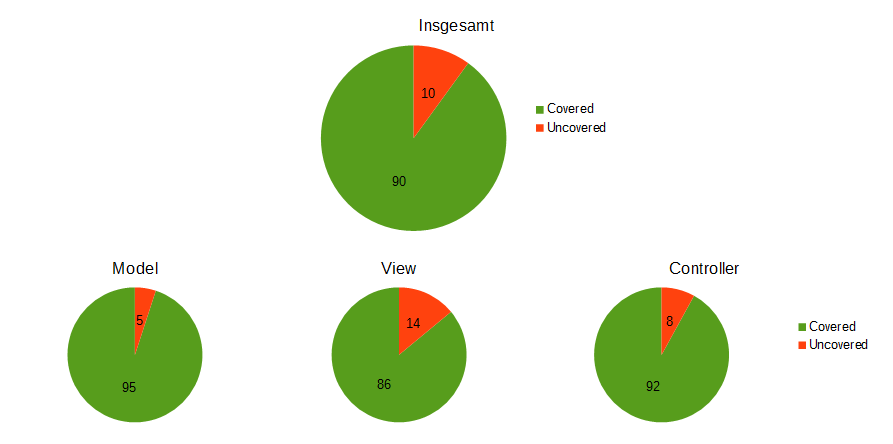
\includegraphics[width=1\linewidth]{img/Testszenarien}
\caption{Testüberdeckung der Testszenarien}
\label{fig:covCoBaB}
\end{figure}
Einerseits wurde die Überdeckung der zuvor beschriebenen, manuell durchgeführten Testszenarien und der Unit Tests bestimmt. Diese Überdeckung kann keine 100\% erreichen, da die Klassen zum Teil Methoden enthalten, die innerhalb von CoBaB nicht aufgerufen werden, sondern nur der Erweiterbarkeit oder besseren Benutzbarkeit für weitere Entwickler dienen. 

\begin{figure}[H]
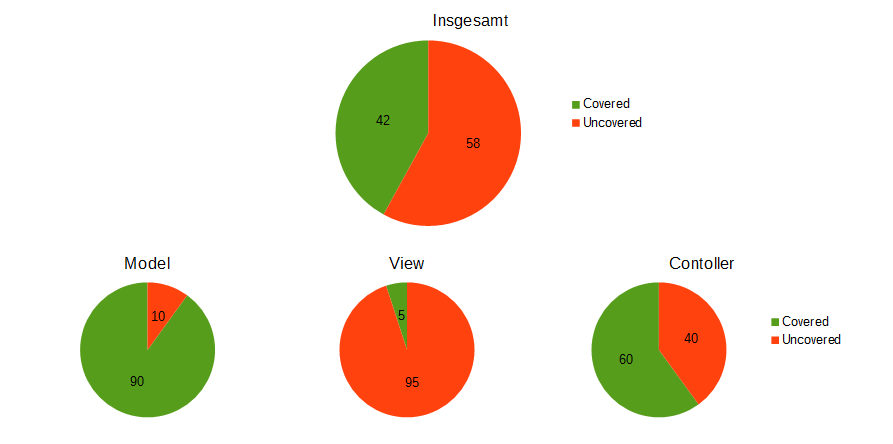
\includegraphics[width=1\linewidth]{img/UnitTests}
\caption{Testüberdeckung der Unit Tests}
\label{fig:covTests}
\end{figure}
Andererseits wurde die Überdeckung der 18 Klassen, die durch Unit Tests getestet wurden, gemessen. Diese Überdeckung ist nicht so hoch, da es für die View-Klassen keine Unit Tests gibt. 


Erzeugen der Ergebnisse:

CoBaB wurde mit OpenCppCoverage gestartet und TS10 ausgeführt:\smallskip\newline
OpenCppCoverage 
-\hspace{1pt}-sources \enquote{Pfad zu CoBaB\textbackslash CoBaB\textbackslash core} 
-\hspace{1pt}-sources \enquote{Pfad zu CoBaB\textbackslash CoBaB\textbackslash interface} 
-\hspace{1pt}-excluded\_sources *.h -\hspace{1pt}-export\_type=binary:CoBaB.cov 
-\hspace{1pt}- \newline \enquote{Pfad zu CoBaB\textbackslash CoBaB\textbackslash build-CoBaB-Desktop\_Qt\_5\_5\_1\_MSVC2013\_64bit-Debug  \textbackslash app\textbackslash debug\textbackslash CoBaB.exe}
\par

CoBaB wurde erneut mit OpenCppCoverage gestartet und TS30-TS90, TSW10-TSW60 und TSW80-TSW120 wurden ausgeführt, ohne CoBaB zu beenden: \smallskip\newline
OpenCppCoverage 
-\hspace{1pt}-sources \enquote{Pfad zu CoBaB\textbackslash CoBaB\textbackslash core} 
-\hspace{1pt}-sources \enquote{Pfad zu CoBaB\textbackslash CoBaB\textbackslash interface} 
-\hspace{1pt}-excluded\_sources *.h -\hspace{1pt}-export\_type=binary:CoBaB1.cov 
-\hspace{1pt}- \enquote{Pfad zu CoBaB\textbackslash CoBaB\textbackslash build-CoBaB-Desktop\_Qt\_5\_5\_1\_MSVC2013\_64bit-Debug \textbackslash app\textbackslash debug\textbackslash CoBaB.exe}
\par

CoBaB wurde mit Kommandozeilenargumenten und OpenCppCoverage gestartet, um TS20 und TSW70 gleichzeitig durchzuführen;\smallskip\newline
OpenCppCoverage 
-\hspace{1pt}-sources \enquote{Pfad zu CoBaB\textbackslash CoBaB\textbackslash core} 
-\hspace{1pt}-sources \enquote{Pfad zu CoBaB\textbackslash CoBaB\textbackslash interface} 
-\hspace{1pt}-excluded\_sources *.h -\hspace{1pt}-export\_type=binary:CoBaB2.cov 
-\hspace{1pt}- \enquote{Pfad zu CoBaB\textbackslash CoBaB\textbackslash build-CoBaB-Desktop\_Qt\_5\_5\_1\_MSVC2013\_64bit-Debug \textbackslash app\textbackslash debug\textbackslash CoBaB.exe} \enquote{Pfad zum Standardordner} -f
\par

Die Unit Tests zu CoBaB wurden ausgeführt und die Überdeckungsergebnisse zusammengefasst:\smallskip\newline
OpenCppCoverage 
-\hspace{1pt}-sources \enquote{Pfad zu CoBaB\textbackslash CoBaB\textbackslash core} 
-\hspace{1pt}-sources \enquote{Pfad zu CoBaB\textbackslash CoBaB\textbackslash interface} 
-\hspace{1pt}-excluded\_sources *.h -\hspace{1pt}-input\_coverage=CoBaB.cov -\hspace{1pt}-input\_ coverage=CoBaB1.cov -\hspace{1pt}-input\_coverage=CoBaB2.cov 
-\hspace{1pt}- \enquote{Pfad zu CoBaB\textbackslash CoBaB\textbackslash build-CoBaB-Desktop\_Qt\_5\_5\_1\_MSVC2013\_64bit-Debug\textbackslash test\textbackslash debug\textbackslash test.exe}
\newline
\par

Die Unit Tests wurden noch einmal alleine ausgeführt, um die Überdeckung nur durch die Unit Tests zu messen: \smallskip\newline
OpenCppCoverage 
-\hspace{1pt}-sources \enquote{Pfad zu CoBaB\textbackslash CoBaB\textbackslash core} 
-\hspace{1pt}-sources \enquote{Pfad zu CoBaB\textbackslash CoBaB\textbackslash interface} 
-\hspace{1pt}-excluded\_sources *.h 
-\hspace{1pt}-excluded\_modules *.dll
-\hspace{1pt}- \enquote{Pfad zu CoBaB\textbackslash CoBaB\textbackslash build-CoBaB-Desktop\_Qt\_5\_5\_1\_MSVC2013\_64bit-Debug \textbackslash test\textbackslash de-bug\textbackslash test.exe}
\par

Da die Ergebnisse von OpenCppCoverage nur die Klassen enthalten, die auch getestet wurden (also nicht die View Klassen), wurde die Überdeckung mithilfe der Ergebnisse der einzelnen Klassen manuell berechnet (überdeckte Zeilen/gesamte Zeilen). Insbesondere, um die Überdeckung von Model, View und Controller zu berechnen.
\pagebreak

\end{document}
